\documentclass[tikz, border=10pt]{standalone}
\usepackage{pgfplots}
\pgfplotsset{compat=1.18}

\begin{document}
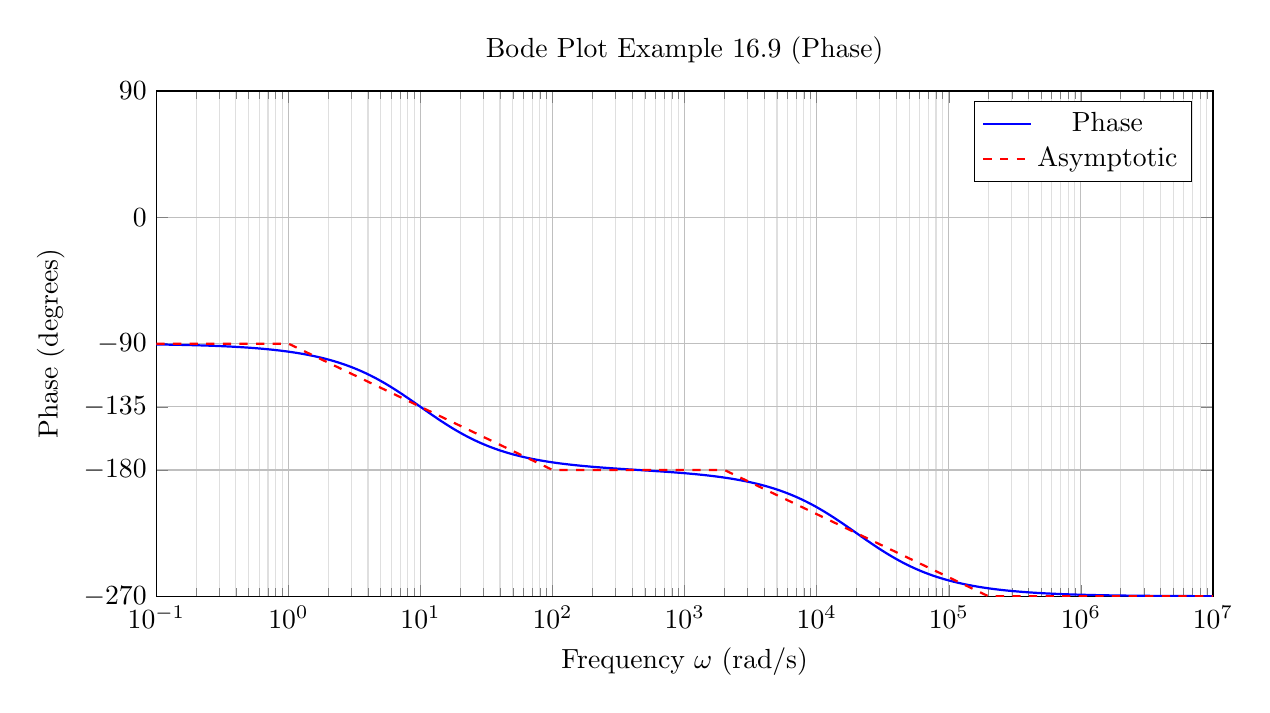
\begin{tikzpicture}
    \begin{semilogxaxis}[
        width=15cm, height=8cm,
        title={Bode Plot Example 16.9 (Phase)},
        xlabel={Frequency $\omega$ (rad/s)},
        ylabel={Phase (degrees)},
        grid=both,
        xmin=0.1, xmax=10000000,
        ymin=-270, ymax=90,
        ytick={90, 0, -90, -135, -180, -270},
        minor grid style={gray!25},
        major grid style={gray!50},
    ]
    % H(s) = -2s / [ (1+s/10)(1+s/20000) ]
    % Phase = angle(-2jw) - angle(1+jw/10) - angle(1+jw/20000)
    % angle(-2jw) = -90 degrees
    % Total Phase = -90 - atan(x/10) - atan(x/20000)
    
    \addplot[blue, thick, domain=0.1:10000000, samples=400] {
        -90 - atan(x/10) - atan(x/20000)
    };
    \addlegendentry{Phase}
    
    % Asymptotes (Approximated)
    % Pole 1 at 10: Starts 0.1*10=1, ends 10*10=100. Slope -45/dec.
    % Pole 2 at 20000: Starts 2000, ends 200000. Slope -45/dec.
    % Base phase: -90
    % Segments:
    % w < 1: -90
    % 1 < w < 100: -90 - 45*log10(x/1)
    % 100 < w < 2000: -90 - 90 = -180
    % 2000 < w < 200000: -180 - 45*log10(x/2000)
    % w > 200000: -180 - 90 = -270
    
    \addplot[red, dashed, thick] coordinates {
        (0.1, -90) (1, -90) (100, -180) (2000, -180) (200000, -270) (10000000, -270)
    };
    \addlegendentry{Asymptotic}

    \end{semilogxaxis}
\end{tikzpicture}
\end{document}
